%\VignetteIndexEntry{HOWTO PROcess}
%\VignettePackage{PROcess}
\documentclass[12pt]{article}

\usepackage{amsmath,pstricks}
\usepackage[authoryear,round]{natbib}
\usepackage{hyperref}


\textwidth=6.2in
\textheight=8.5in
%\parskip=.3cm
\oddsidemargin=.1in
\evensidemargin=.1in
\headheight=-.3in

\newcommand{\scscst}{\scriptscriptstyle}
\newcommand{\scst}{\scriptstyle}

\bibliographystyle{plainnat}
%\bibliographystyle{apalike}

\usepackage{/scratch/homes/xiaochun/R/share/texmf/Sweave}
\begin{document}

\title{HowTo Use the Bioconductor PROcess package}
\author{}
\maketitle
\tableofcontents

% library(tools)
% Rnwfile<- file.path("~/PROcess/inst/doc","howtoprocess.Rnw")
% Sweave(Rnwfile,pdf=TRUE,eps=TRUE,stylepath=TRUE,driver=RweaveLatex())

\section{Introduction}
The {\tt PROcess} package contains a collection of functions for 
processing spectra to remove baseline drifts if any, detect
peaks and align them to a set of protobiomarkers. This document 
serves as a quick tutorial for using the {\tt PROcess} package.

\section{Baseline subtraction}
Our first observation of a raw spectrum is that it exhibits
elevated baseline, more so at smaller m/z values than at larger
values. This elevated baseline
is mostly caused by the chemical noises in the EAM and ion
overload. Ideally a spectrum should rest more
or less on the zero horizontal line.  This baseline needs to
be subtracted from each raw spectrum. The following example 
shows the result of a spectrum with its baseline removed. 

\begin{Schunk}
\begin{Sinput}
> library(PROcess)
\end{Sinput}
\begin{Soutput}
Loading required package: Icens 
\end{Soutput}
\begin{Sinput}
> fdat <- system.file("Test", package = "PROcess")
> fs <- list.files(fdat, pattern = "*csv*", full.names = TRUE)
> f1 <- read.files(fs[1])
> fcut <- f1[f1[, 1] > 0, ]
> bseoff <- bslnoff(fcut, method = "loess", plot = TRUE, bw = 0.1)
> title(basename(fs[1]))
\end{Sinput}
\end{Schunk}
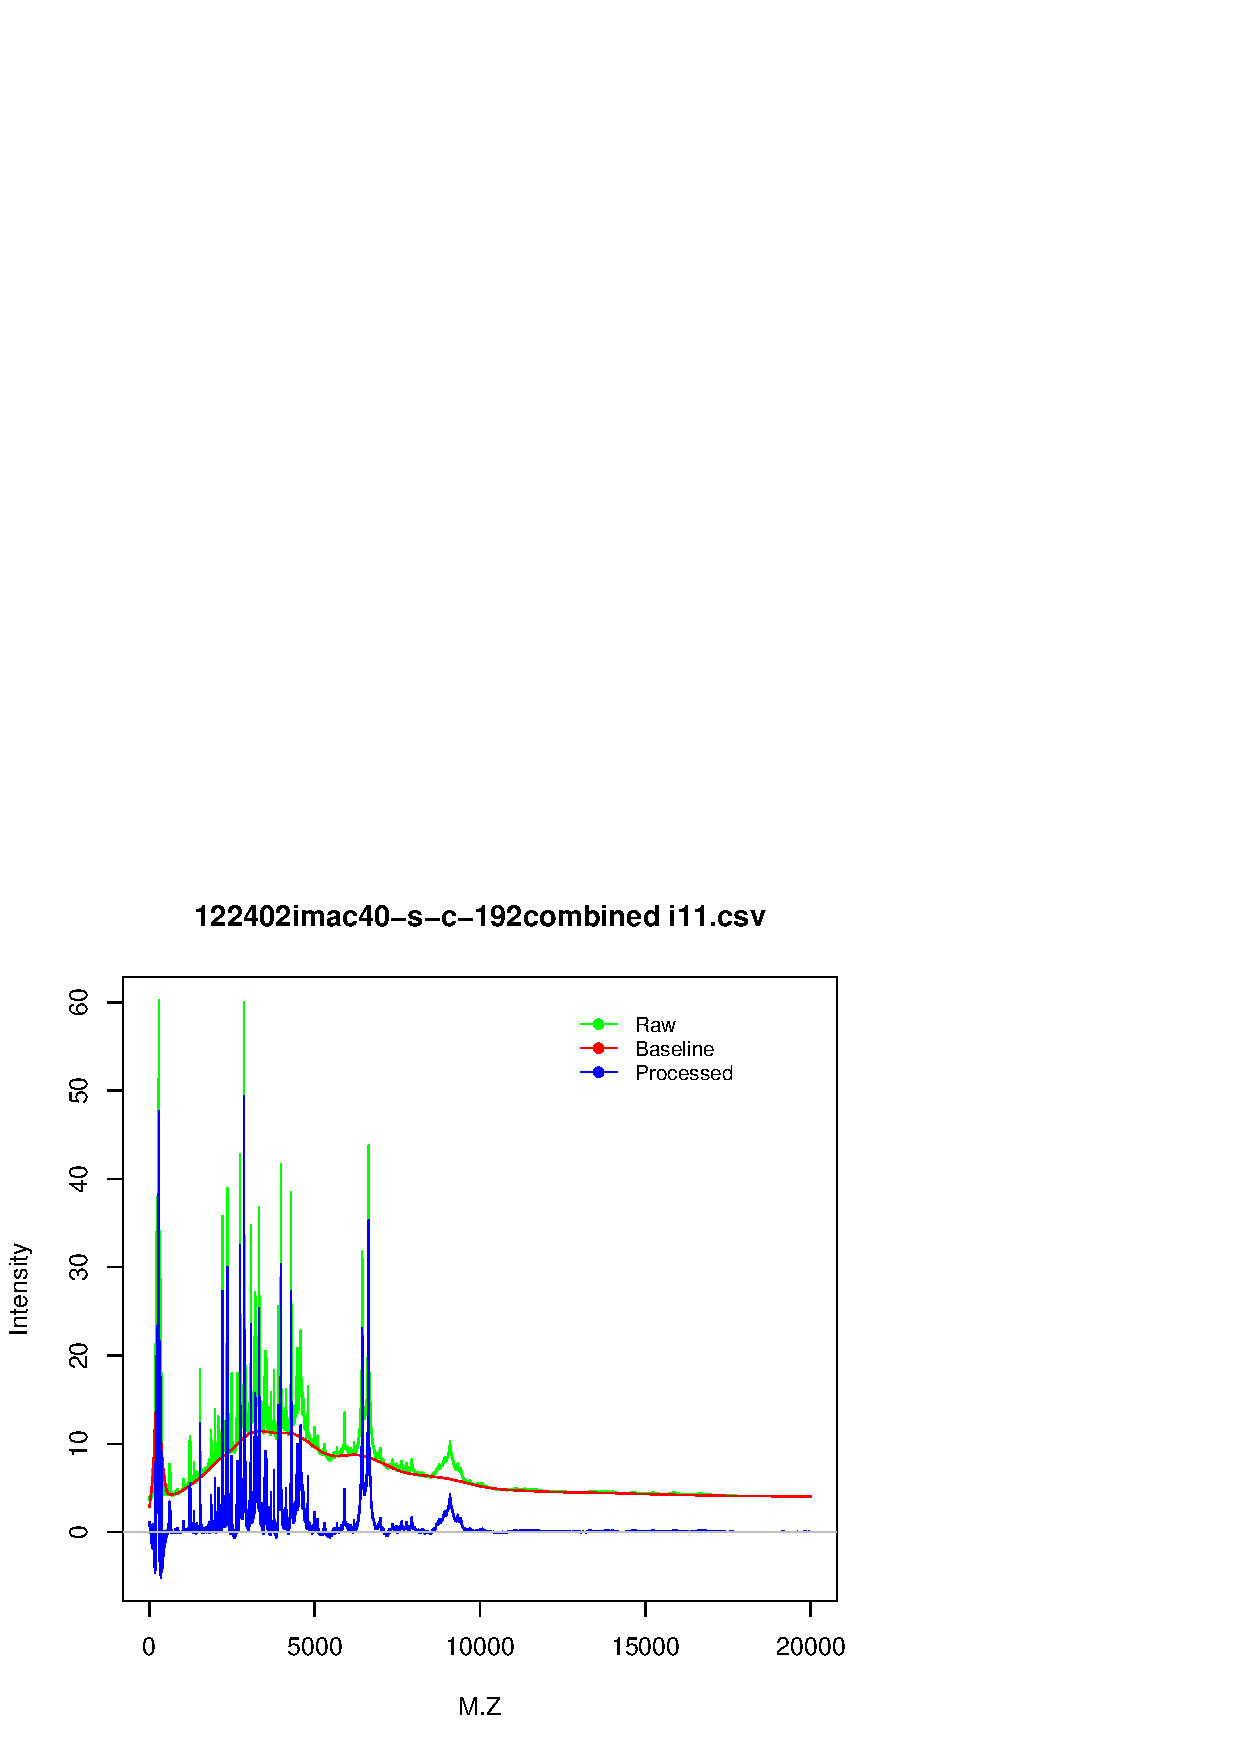
\includegraphics{howtoprocess-bslnoffSingle}
\section{Peak detection}
After baseline is removed, peaks can be located by using
{\tt isPeak}. A spectrum is smoothed first using moving 
average of the $k$ nearest neighbours. Smoothing helps 
to enhance peaks and get rid of spurious peaks. However, we 
do not recommend large amount of smoothing (controlled by
parameter {\tt sm.span}) in this step because we do not 
wish to 
smooth away too many short and wide peaks 
and also we need the precision in peak locations. As a first step 
we do not mind getting more potential features. 

\begin{Schunk}
\begin{Sinput}
> pkgobj <- isPeak(bseoff, span = 81, sm.span = 11, plot = TRUE)
\end{Sinput}
\end{Schunk}
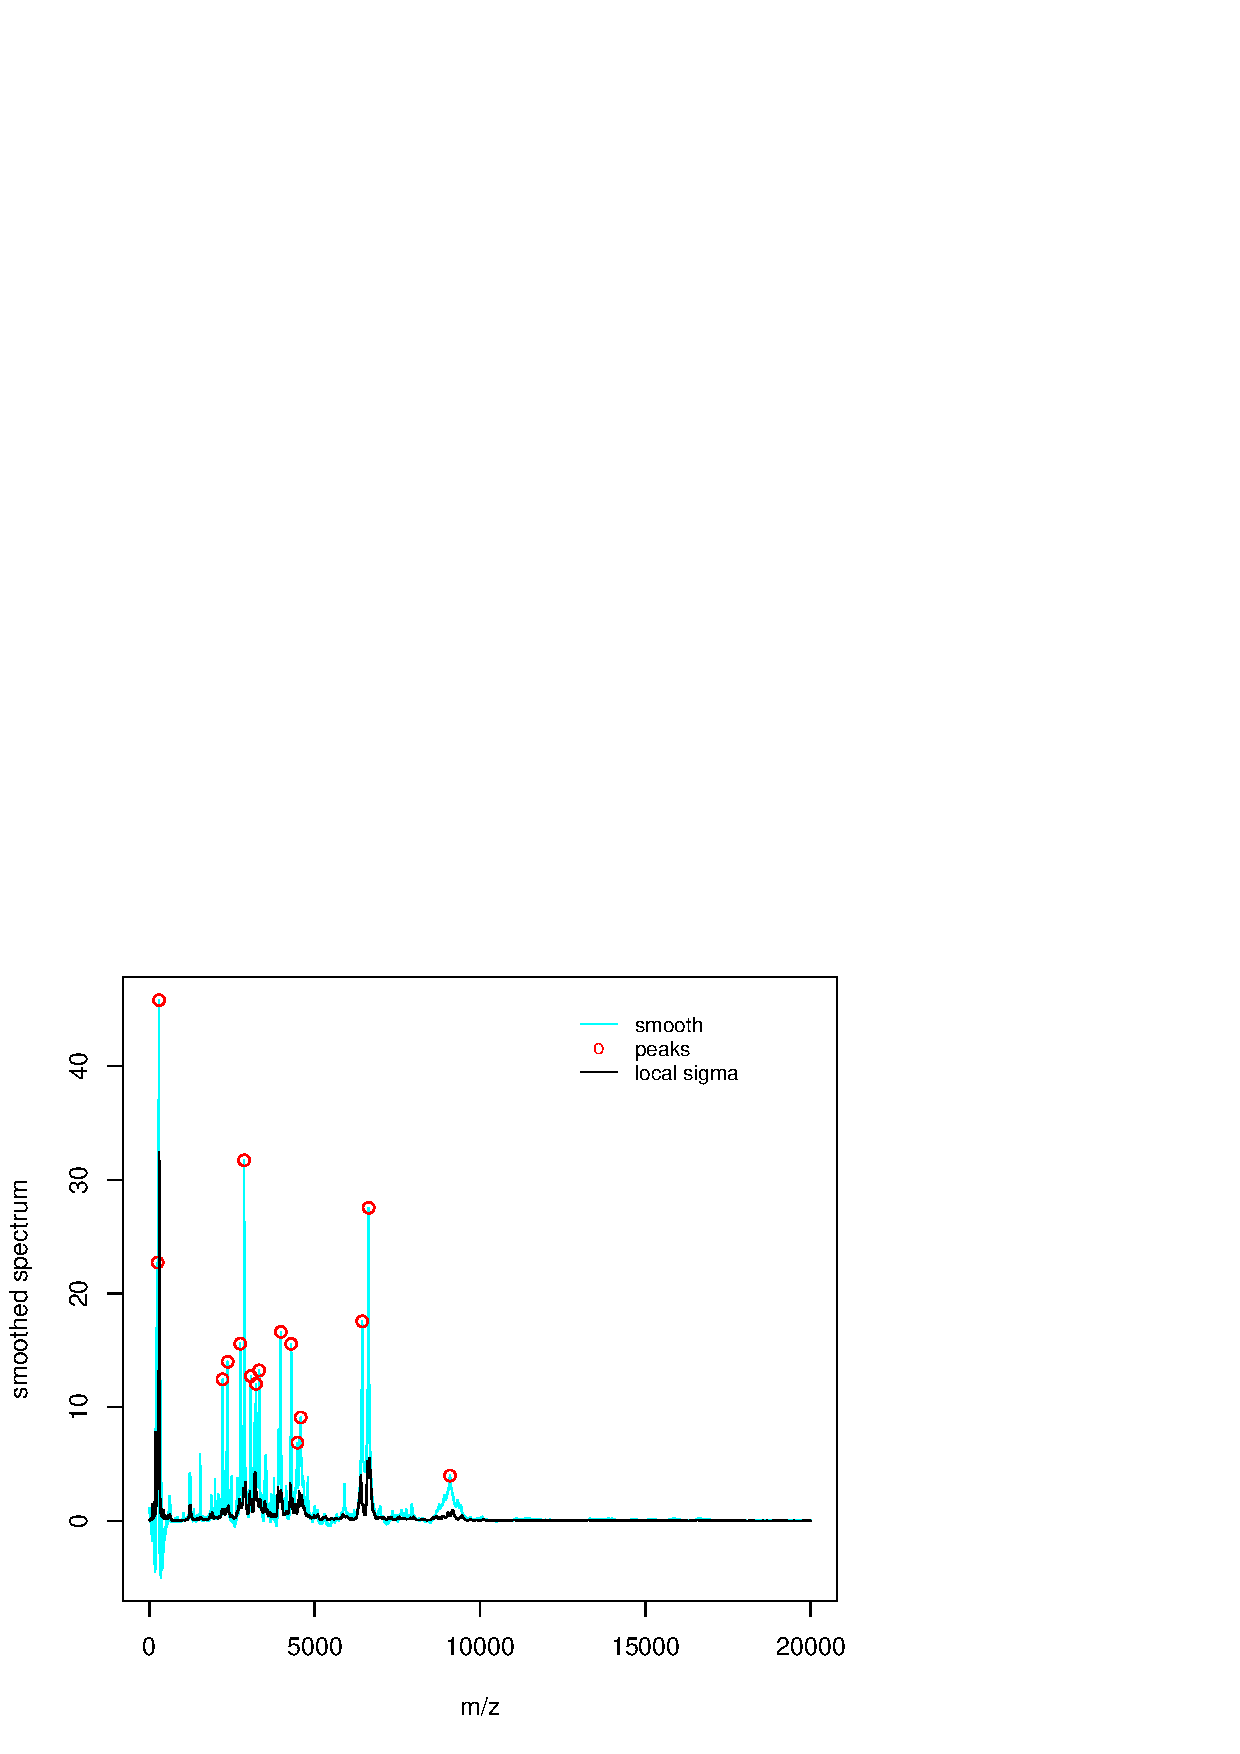
\includegraphics{howtoprocess-isPeakSingle}

We can also zoom in to inspect peaks in a particular range of 
m/z values.
\begin{Schunk}
\begin{Sinput}
> specZoom(pkgobj, xlim = c(5000, 10000))
\end{Sinput}
\end{Schunk}
\includegraphics{howtoprocess-specZoom}

\section{Batch operation}
We demonstrate the batch functionality of this package using
a set of 2 spectra.
\subsection{Apply baseline subtraction to a set of spectra}
\begin{Schunk}
\begin{Sinput}
> testdir <- system.file("Test", package = "PROcess")
> testM <- rmBaseline(testdir)
\end{Sinput}
\end{Schunk}

\subsection{Renormalize spectra}
Suppose we want to normalize a set of spectra to their median 
AUC (Area Under the Curve), where an AUC is calculated for
m/z values greater than a cutoff point, 1500.

\begin{Schunk}
\begin{Sinput}
> rtM <- renorm(testM, cutoff = 1500)
\end{Sinput}
\end{Schunk}

\subsection{Identify peaks of spectra}
\begin{Schunk}
\begin{Sinput}
> peakfile <- paste(tempdir(), "testpeakinfo.csv", sep = "/")
> getPeaks(testM, peakfile)
\end{Sinput}
\end{Schunk}

\subsection{Quality assessment}
Quality assessment is necessary because some spectra are very 
noisy and have hardly any peaks. Function {\tt quality} 
computes three parameters {\tt Quality}, {\tt Retain} and 
{\tt peak} for assessing a set of spectra.
\begin{Schunk}
\begin{Sinput}
> qualRes <- quality(testM, peakfile, cutoff = 1500)
> print(qualRes)
\end{Sinput}
\begin{Soutput}
                                       Quality    Retain peak
122402imac40-s-c-192combined i11.csv 0.5419809 0.3825606 1.28
122402imac40-s-c-192combined i12.csv 0.6234699 0.3548255 0.72
\end{Soutput}
\end{Schunk}

A spectrum is deemed of poor quality and should be removed from
subsequent analyses if it meets the following 3
conditions simultaneously:
\begin{enumerate}
\item $\mbox{\tt Quality}\, <\, 0.4$;
\item $\mbox{\tt Retain}\, <\, 0.1 $;
\item $\mbox{\tt peak} \,< \,1/2 \mbox{ of the mean peak number in the
chip}$.
\end{enumerate}


\subsection{Get protobiomarkers}
One challenge in MS data is that not only they exhibit
variation vertically but also do they horizontally. This
horizontal variation is not simply a constant shift but
associated with value of m/z. Currently the 
accuracy in the m/z position is believed to be within $0.3\%$ o
f the m/z value. Once the peaks are detected, we align the
peaks by first generating an interval of size $0.3\%$ of 
the m/z value which centers at m/z for each m/z where a peak is 
detected. We treat those m/z
intervals as interval censored data. Maximum likelihood 
estimate
of the distribution of survival times conditional upon the 
observed intervals  can be computed by the method of
\cite{Gent:Geye:1994}. Protobiomarkers are computed as 
the center
of the MLE intervals. For a spectrum whose peaks are in the
clique that define a protobiomarker, its value at this 
protobiomarker
is set to be the maximum of the peaks in the clique, otherwise
its value is set to be the value of its nearest neighbour.


\begin{Schunk}
\begin{Sinput}
> bmkfile <- paste(tempdir(), "testbiomarker.csv", sep = "/")
> testBio <- pk2bmkr(peakfile, testM, bmkfile)
> mzs <- as.numeric(rownames(rtM))
> matplot(mzs, rtM, type = "l", xlim = c(1000, 10000), ylab = "intensities", 
+     main = "proto-biomarkers")
> bks <- getMzs(testBio)
> abline(v = bks, col = "green")
\end{Sinput}
\end{Schunk}
\includegraphics{howtoprocess-pk2bmkr}
\bibliography{howtoprocess}

\end{document}

